% !TEX root = task-3-11-3.tex
% Editable task bank. Append new BankTask blocks at the end of the document.
\documentclass[12pt,a4paper]{article}
\usepackage{physics-textbook}
\usepackage{graphicx,needspace}
\usetikzlibrary{decorations.pathmorphing}
\newif\ifShowSolutions
\ifdefined\TutorEdition
  \ShowSolutionstrue
\else
  \ShowSolutionsfalse % Change to \ShowSolutionstrue to display solutions.
\fi
\newcounter{banktask}
\newsavebox{\BankTaskBox}
\newcommand{\BankTaskContent}[3]{%
  \noindent\textbf{\thebanktask.}\quad #2\par
  \ifShowSolutions
    \Needspace{50mm}% Keep the solution heading with its opening text or diagram.
    #3\par
    \ifdefined\TutorEdition
      \ifcsname TutorSource#1\endcsname
        \nopagebreak\smallskip{\small\csname TutorSource#1\endcsname\par}%
      \fi
    \fi
  \fi
}
\newcommand{\BankTask}[3]{%
  \refstepcounter{banktask}\par\medskip
  \sbox{\BankTaskBox}{\begin{minipage}{\linewidth}%
    \BankTaskContent{#1}{#2}{#3}\end{minipage}}%
  \ifdim\dimexpr\ht\BankTaskBox+\dp\BankTaskBox\relax>\dimexpr\textheight-20mm\relax
    \Needspace{35mm}\BankTaskContent{#1}{#2}{#3}%
  \else
    \Needspace{\dimexpr\ht\BankTaskBox+\dp\BankTaskBox\relax}%
    \noindent\usebox{\BankTaskBox}\par
  \fi
  \medskip
}
\begin{document}
\BookSubsection{3.11.3}{Закон Джоуля–Ленца}


% Source sdamgia-1406: https://phys-ege.sdamgia.ru/problem?id=1406
\BankTask{sdamgia-1406}{
Чему равно время прохождения тока силой $5$ А по проводнику, если при напряжении на его концах $120$ В в проводнике выделяется количество теплоты, равное $540$ кДж? (Ответ дайте в секундах.)
}{
\smallskip\noindent\textbf{Решение}\par
Согласно закону Джоуля — Ленца количество выделяемого тепла в проводнике определяется выражением $Q=UIt.$ Отсюда находим время прохождения тока по проводнику:

\[t= \frac{Q}{UI} = \frac{540\,\text{\,\text{кДж}}}{120\,\text{В} \cdot  5\,\text{А}} = \frac{540 \cdot  10 ^3\,\text{Дж}}{120\,\text{В} \cdot  5\,\text{А}} =900\,\text{с}.\]

Ответ: $900$.
}

% Source sdamgia-1418: https://phys-ege.sdamgia.ru/problem?id=1418
\BankTask{sdamgia-1418}{
В электронагревателе с неизменным сопротивлением спирали, через который течет постоянный ток, за время $t$ выделяется количество теплоты Q. Если силу тока и время $t$ увеличить вдвое, то во сколько раз увеличится количество теплоты, выделившееся в нагревателе?
}{
\smallskip\noindent\textbf{Решение}\par
Согласно закону Джоуля — Ленца, количество теплоты, выделяющееся на спирали электронагревателя при прохождении тока, пропорционально произведению квадрата силы тока и времени прохождения тока: $Q=I ^2 Rt.$ Следовательно, увеличение силы тока и времени его прохождения в $2$ раза приведет к увеличению количества теплоты в $8$ раз.

Ответ: $8$.
}

% Source sdamgia-1428: https://phys-ege.sdamgia.ru/problem?id=1428
\BankTask{sdamgia-1428}{
Резистор $1$ с электрическим сопротивлением $3$ Ом и резистор $2$ с электрическим сопротивлением $6$ Ом включены последовательно в цепь постоянного тока. Чему равно отношение количества теплоты, выделяющегося на резисторе $1$, к количеству теплоты, выделяющемуся на резисторе $2$ за одинаковое время?
}{
\smallskip\noindent\textbf{Решение}\par
Согласно закону Джоуля — Ленца, количество теплоты, выделяющееся на проводнике при прохождении тока, пропорционально произведению квадрата силы тока, величины сопротивления проводника и времени прохождения тока: $Q=I ^2 Rt.$ Поскольку резисторы подключены последовательно, ток через них течет одинаковый, а значит, отношение количества теплоты, выделяющегося на резисторе $1$, к количеству теплоты, выделяющемуся на резисторе $2$, за одинаковое время равно: 

\[\frac{Q_1}{Q_2} = \frac{I^2R_1t}{I^2R_2t}= \frac{R_1}{R_2} = \frac{3\,\text{Ом}}{6\,\text{Ом}} =0{,}5.\]

Ответ: $0{,}5$.
}

% Source sdamgia-4910: https://phys-ege.sdamgia.ru/problem?id=4910
\BankTask{sdamgia-4910}{
Комната освещается четырьмя одинаковыми параллельно включенными лампочками. Расход электроэнергии за час равен Q. Каким должно быть число параллельно включенных лампочек, чтобы расход электроэнергии в час был равен $2$Q?
}{
\smallskip\noindent\textbf{Решение}\par
При параллельном соединении ко всем лампочкам приложено одинаковое напряжение $U.$ Независимо от общего количества лампочек за $1$ час каждая лампочка расходует одинаковое количество энергии $\frac{U ^2}{R} \cdot  1\,\text{ч},$ где $R$ — сопротивление лампочки. Согласно условию, расход $4$ лампочек равен $Q=4 \cdot  \frac{U ^2}{R} \cdot  1\,\text{ч}.$ Следовательно, чтобы расход энергии за час стал равен $2Q,$ необходимо, чтобы было включено $8$ лампочек (параллельно соединенных).

Ответ: $8$.
}

% Source sdamgia-42639: https://phys-ege.sdamgia.ru/problem?id=42639
\BankTask{sdamgia-42639}{
При прохождении по проводнику постоянный электрический ток силой $3$ А в течение $60\,\text{с}$ совершает работу, равную $270$ кДж. Чему равно сопротивление проводника? Ответ запишите в омах.
}{
\smallskip\noindent\textbf{Решение}\par
Из формулы работы электрического тока $A=I ^2 Rt$ находим сопротивление проводника:

\[R= \frac{A}{I ^2 t} = \frac{270000}{9 \cdot  60} =500\,\text{Ом}.\]

Ответ: $500$.
}

% Source sdamgia-46771: https://phys-ege.sdamgia.ru/problem?id=46771
\BankTask{sdamgia-46771}{
Паяльник подключили к источнику постоянного напряжения $220$ В. Какое количество теплоты выделится за $20$ минут работы паяльника, если сила тока в цепи его питания равна $1{,}2$ А? Ответ дайте в килоджоулях.
}{
\smallskip\noindent\textbf{Решение}\par
Количество теплоты, выделяющееся в проводнике при прохождении тока равно работе тока

\[Q = UIt = 220 \cdot  1{,}2 \cdot  1200 = 316800\,\text{Дж} = 316{,}8\,\text{\,\text{кДж}}.\]

Ответ: $316{,}8$.
}

% Source sdamgia-9741: https://phys-ege.sdamgia.ru/problem?id=9741
\BankTask{sdamgia-9741}{
Два последовательно соединенных резистора сопротивлениями $4$ Ом и $8$ Ом подключены к аккумулятору, напряжение на клеммах которого равно $24$ В. Какая тепловая мощность выделяется в резисторе большего номинала?
}{
\smallskip\noindent\textbf{Решение}\par
Резисторы подключены последовательно, а, значит, полное сопротивление цепи представляет собой сумму сопротивлений резисторов. По закону Ома в цепи течет ток, по величине равный:

$I = \frac{U}{R} = \frac{24}{4 + 8} =2$ А.

На резисторе с большим сопротивлением выделится тепловая мощность:

$P=I ^2 R=2 ^2 \cdot  8 = 32$ Вт.

Ответ: $32$.
}

% Source sdamgia-24103: https://phys-ege.sdamgia.ru/problem?id=24103
\BankTask{sdamgia-24103}{
Лампа накаливания подключена к источнику напряжения. После увеличения напряжения на лампе в $3$ раза выделяющаяся в ней мощность возросла в $6$ раз. Во сколько раз при этом увеличилось сопротивление спирали лампы? Ответ округлите до десятых долей.
}{
\smallskip\noindent\textbf{Решение}\par
По условию $U_{2}$ = $3$$U_{1}$, а $P_{2}$ = $6$$P_{1}$. Из формулы мощности $P= \frac{U ^2}{R} \Rightarrow R= \frac{U ^2}{P} .$ Отсюда находим отношение сопротивлений $\frac{R_2}{R_1} = \frac{9}{6} =1{,}5.$

Ответ: $1{,}5$.
}

% Source sdamgia-35994: https://phys-ege.sdamgia.ru/problem?id=35994
\BankTask{sdamgia-35994}{
Через первый резистор сопротивлением $R$ течет постоянный электрический ток силой I. Через второй резистор сопротивлением $8$R течет постоянный электрический ток силой $\frac{I}{2} .$ Чему равно отношение мощностей $\frac{P_2}{P_1} ,$ выделяющихся во втором и в первом резисторах?
}{
\smallskip\noindent\textbf{Решение}\par
Мощность тока определяется по формуле $P = I ^2 R.$ Тогда отношение мощностей равно:

\[\frac{P_2}{P_1} = \frac{I ^2 \cdot  8R}{4I ^2 \cdot  R} = 2.\]

Ответ: $2$.
}

% Source sdamgia-31890: https://phys-ege.sdamgia.ru/problem?id=31890
\BankTask{sdamgia-31890}{
К концам длинного цилиндрического однородного провода приложено напряжение U. Провод укоротили вдвое, а приложенное напряжение уменьшили в $2$ раза. Как в результате изменятся при этом сила тока в проводе и выделяющаяся в нем мощность?

Для каждой величины определите соответствующий характер изменения.

$1$. Увеличится.

$2$. Уменьшится.

$3$. Не изменится.

 

\begin{center}\small\renewcommand{\arraystretch}{1.25}\begin{tabular}{|p{0.450\linewidth}|p{0.450\linewidth}|}\hline
Сила тока & Мощность, выделяющаяся в проводе\\\hline
 & \\\hline
\end{tabular}\end{center}
}{
\smallskip\noindent\textbf{Решение}\par
При уменьшении длины проводника в $2$ раза его сопротивление уменьшится в $2$ раза. Сила тока по закону Ома для участка цепи $I= \frac{U}{R}$ при уменьшении напряжения и сопротивления в $2$ раза не изменится ($3$).

Мощность тока $P=I ^2 R$ соответственно уменьшится в $2$ раза ($2$).

Ответ: $32$.
}


% Source 0990BD: https://ege.fipi.ru/bank/questions.php?search=1&proj=BA1F39653304A5B041B656915DC36B38&qid=0990BD
\BankTask{0990BD}{
При прохождении по проводнику постоянный электрический ток силой $3\,\text{А}$ в течение $60\,\text{с}$ совершает работу, равную $270\,\text{кДж}$. Чему равно сопротивление проводника (в $\text{Ом}$)?
}{
\smallskip\noindent\textbf{Решение от GPT}\par
Работа постоянного тока $A=I^2Rt$. Следовательно,
\[
R=\frac{A}{I^2t}=\frac{270\cdot10^3}{3^2\cdot60}=500\,\text{Ом}.
\]
Ответ: $500\,\text{Ом}$.
}

% Source 8025: https://phys-ege.sdamgia.ru/problem?id=8025
\BankTask{8025}{
\begin{center}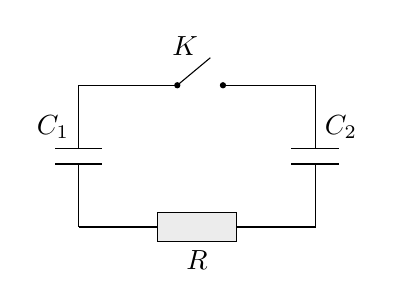
\begin{tikzpicture}[>=stealth]

\draw(0,0)--(1,0) (2,0)--(3,0)--(3,.8) (3,1)--(3,1.8)--(1.83,1.8) (1.25,1.8)--(0,1.8)--(0,1) (0,.8)--(0,0);
\draw(-.3,.8)--(.3,.8) (-.3,1)--(.3,1) (2.7,.8)--(3.3,.8) (2.7,1)--(3.3,1);
\draw[fill=gray!15](1,-.18)rectangle(2,.18);\draw(1.25,1.8)--(1.67,2.15);
\fill (1.25,1.8)circle(.04) (1.83,1.8)circle(.04);\node[above]at(1.35,2.05){$K$};\node[above left]at(0,1){$C_1$};\node[above right]at(3,1){$C_2$};\node[below]at(1.5,-.18){$R$};
\end{tikzpicture}\end{center}
Конденсатор $C_{1}$  =  $1$ мкФ заряжен до напряжения U  =  $300\,\text{В}$ и включен в последовательную цепь из резистора R  =  $300\,\text{Ом}$, незаряженного конденсатора $C_{2}$  =  $2$ мкФ и разомкнутого ключа К (см. рис.). Какое количество теплоты выделится в цепи после замыкания ключа, пока ток в цепи не прекратится?
}{
\smallskip\noindent\textbf{Решение}\par
После соединения конденсаторов напряжение U на них будет одинаковым. По закону сохранения заряда $q_1 + q_2=q_1' + q_2',$ где заряды до соединения на первом конденсаторе равен $q_1=C_1U_1,$ на втором конденсаторе $q_2=0,$ а заряды после соединения $q_1'=C_1U$ и $q_2'=C_2U.$ Откуда получаем:

\[C_1U_1=U ( C_1 + C_2 ) .\]

Энергии конденсаторов до и после соединения равнялись $W_1= \frac{C_1U_1 ^2}{2}$ и $W_2= \frac{( C_1 + \,\text{С}_2 ) U ^2}{2} .$ Выделившаяся на резисторе теплота равна $Q=W_1 - W_2.$
По закону сохранения энергии выделившееся в цепи количество теплоты равно разности значений энергии конденсаторов в начальном и конечном состояниях: 

\[Q= \frac{C_1U ^2}{2} - \frac{( C_1U ) ^2}{2 ( C_1 + C_2 )} .\]

Откуда получим:

\[Q= \frac{C_1C_2U ^2}{2 ( C_1 + C_2 )} = \frac{10 ^{ - 6 } \cdot 2 \cdot 10 ^{ - 6 } \cdot 300 ^2}{2 ( 10 ^{ - 6 } + 2 \cdot 10 ^{ - 6 } )} =0{,}03\,\text{Дж}.\]

Ответ: Q  =  $30\,\text{мДж}$.
}

% Source 11955: https://phys-ege.sdamgia.ru/problem?id=11955
\BankTask{11955}{
\begin{center}\begin{tikzpicture}[>=stealth]

\draw[step=.5,gray!55] (0,-1.5)grid(3,2.5);
\draw[->] (0,-1.5)--(0,2.58) node[above left]{$B_{\text{п}},\,\text{Тл}$};\draw[->] (0,0)--(3.08,0) node[right]{$t,\,\text{с}$};
\draw[thick](0,1.5)--(1,-1)--(2.5,.5);\node[below left] at(0,0){$0$};
\foreach \y/\t in {-.5/{-0{,}2},-1/{-0{,}4},.5/{0{,}2},1/{0{,}4},1.5/{0{,}6}}{\node[left]at(0,\y){$\t$};}
\node[below]at(1,0){$4$};\node[below]at(2,0){$8$};
\end{tikzpicture}\end{center}
Квадратная проволочная рамка со стороной l  =  $10\,\text{см}$ находится в однородном магнитном поле с индукцией $\vec{B}.$ На рисунке изображена зависимость проекции вектора $\vec{B}$ на перпендикуляр к плоскости рамки от времени. Какое количество теплоты выделится в рамке за время t  =  $10\,\text{с}$, если сопротивление рамки R  =  $0{,}2\,\text{Ом}$?
}{
\smallskip\noindent\textbf{Решение}\par
При изменении магнитного поля изменяется поток вектора магнитной индукции $\,\text{Ф} ( t ) = B ( t ) S$ через рамку площадью $S = l ^2 ,$ что создает в ней ЭДС индукции $\mathcal E.$ В соответствии с законом индукции Фарадея:

\[\mathcal E = - \frac{\Delta \,\text{Ф}}{\Delta t} .\]

Эта ЭДС вызывает в рамке ток, сила которого определяется законом Ома для замкнутой цепи: 

\[I= \frac{\mathcal E}{R} .\]

Согласно закону Джоуля  — Ленца за время $\Delta$t в рамке выделится количество теплоты:

\[Q = I ^2 R\Delta t .\]

Таким образом, количество теплоты, выделяющееся в рамке, равно:

\[Q= \frac{l ^{4}}{R} \cdot \frac{( \Delta B_n ) ^2}{\Delta t} .\]

На первом участке графика $\Delta t = t_1 = 4\,\text{с}$ и $\Delta B = B_1 - B_0 = - 1\,\text{Тл},$ на втором участке $\Delta t_2 = t_2 - t_1 = 6\,\text{с}$ и $\Delta B = B_2 - B_1 = 0{,}6\,\text{Тл},$ поэтому суммарное количество выделившейся теплоты:

\[Q = Q_1 + Q_2 = \frac{l ^{4}}{R} \left[ \frac{( \Delta B_1 ) ^2}{\Delta t_1} + \frac{( \Delta B_2 ) ^2}{\Delta t_2} \right] .\]

Подставляя сюда значения физических величин, получим:

\[Q = \frac{( 0{,}1\,\text{м} ) ^{4}}{0{,}2\,\text{Ом}} \cdot \left[ \frac{1\,\text{Тл} ^2}{4\,\text{с}} + \frac{0{,}36\,\text{Тл} ^2}{6\,\text{с}} \right] = 0{,}155 \cdot 10 ^{ - 3 } \,\text{Дж}.\]

Ответ: $0{,}155\,\text{мДж}$.
}

% Source 4756: https://phys-ege.sdamgia.ru/problem?id=4756
\BankTask{4756}{
\begin{center}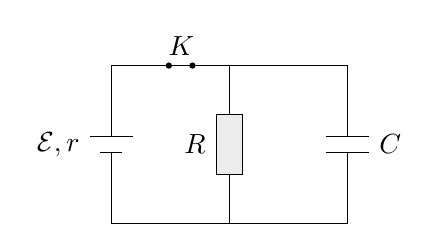
\begin{tikzpicture}[>=stealth]

\draw(0,0)--(3,0)--(3,.9) (3,1.1)--(3,2)--(1.03,2) (.73,2)--(0,2)--(0,1.1) (0,.9)--(0,0);
\draw(.73,2)--(1.03,2);\fill(.73,2)circle(.04) (1.03,2)circle(.04);\node[above]at(.89,2){$K$};
\draw(-.27,1.1)--(.27,1.1) (-.14,.9)--(.14,.9) (2.73,1.1)--(3.27,1.1) (2.73,.9)--(3.27,.9);
\draw(1.5,0)--(1.5,.62) (1.5,1.38)--(1.5,2);\draw[fill=gray!15](1.33,.62)rectangle(1.67,1.38);
\node[left]at(-.28,1){$\mathcal E,r$};\node[left]at(1.32,1){$R$};\node[right]at(3.28,1){$C$};
\end{tikzpicture}\end{center}
В электрической схеме, показанной на рисунке, ключ К замкнут. ЭДС батарейки $\mathcal E = 12\,\text{В},$ емкость конденсатора $C = 0{,}2\,\text{мкФ}.$ Отношение внутреннего сопротивления батарейки к сопротивлению резистора $k= \frac{r}{R} =0{,}2.$ Найдите количество теплоты, которое выделится на резисторе после размыкания ключа К в результате разряда конденсатора.
}{
\smallskip\noindent\textbf{Решение}\par
Когда ключ замкнут, конденсатор заряжен, а через резистор течет ток, который можно найти, применив закон Ома для полной цепи:

\[I= \frac{\mathcal E}{R + r} .\]

Поскольку резистор и конденсатор подключены параллельно, напряжения на них совпадают и равны:

\[U = IR = \frac{R \mathcal E}{R + r} .\]

После размыкания ключа, конденсатор разряжается через сопротивление, и вся накопленная в нем энергия электрического поля переходит в тепло. Таким образом, искомое количество теплоты равно:

\[Q= \frac{CU ^2}{2} = \frac{C}{2} ( \frac{\mathcal E}{1 + r/R} ) ^2 = \frac{0{,}2 \cdot 10 ^{ - 6 } \,\text{Ф}}{2} \cdot ( \frac{12\,\text{В}}{1 + 0{,}2} ) ^2 = 10 ^{ - 5 } \,\text{Дж}.\]

Ответ: $10 ^{ - 5 } \,\text{Дж}.$
}

% Source 32269: https://phys-ege.sdamgia.ru/problem?id=32269
\BankTask{32269}{
\begin{center}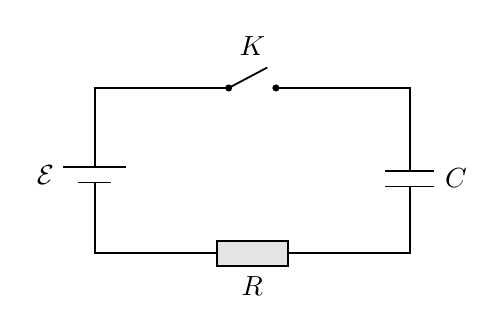
\begin{tikzpicture}[>=stealth,line width=.65pt]\draw (0,1.1)--(0,2.1)--(1.7,2.1) (2.3,2.1)--(4,2.1)--(4,1.05) (4,.85)--(4,0)--(2.45,0) (1.55,0)--(0,0)--(0,.9);\draw (-.4,1.1)--(.4,1.1) (-.21,.9)--(.21,.9) (3.69,1.05)--(4.31,1.05) (3.69,.85)--(4.31,.85);\draw (1.7,2.1)--(2.19,2.36);\foreach \x in {1.7,2.3}{\fill (\x,2.1) circle (.045);}\draw[fill=gray!20](1.55,-.16)rectangle(2.45,.16);\node[left]at(-.39,1){$\mathcal E$};\node[right]at(4.32,.95){$C$};\node[below]at(2,-.17){$R$};\node[above]at(2,2.38){$K$};\end{tikzpicture}\end{center}

Незаряженный конденсатор с емкостью C  =  $0{,}1$ мкФ подключают к источнику тока по схеме, показанной на рисунке. Сопротивление резистора R  =  $500\,\text{Ом}$, сопротивлением проводов и внутренним сопротивлением источника можно пренебречь. После замыкания ключа К на резисторе выделяется тепло равное $7{,}2$ мкДж. Чему равно ЭДС источника?
}{
\smallskip\noindent\textbf{Решение}\par
При замыкании цепи через резистор проходит ток зарядки до тех, пока конденсатор не зарядится до напряжения, равного ЭДС источника тока.
При этом через источник тока протечет заряд, равный $q=CU=C \mathcal{E} .$ Тогда в источнике тока будет совершена работа $A=q \mathcal{E} =C \mathcal{E} ^2 .$
Энергия, которую приобретет при этом заряженный конденсатор, равна:

\[W_{\,\text{р}}= \frac{CU ^2}{2} = \frac{C \mathcal{E} ^2}{2} .\]

Поскольку сопротивлением проводов и внутренним сопротивлением источника тока можно пренебречь, то можно применить закон сохранения энергии:

$A_{\,\text{ист}}=Q + W_p,$
$C \mathcal{E} ^2 =Q + \frac{C \mathcal{E} ^2}{2} ,$

 откуда:

\[\mathcal E=\sqrt{\frac{2Q}{C}}=\sqrt{\frac{2\cdot7{,}2\cdot10^{-6}}{0{,}1\cdot10^{-6}}}=12\,\text{В}.\]

Ответ: $12\,\text{В}$.
}

% Source 42802: https://phys-ege.sdamgia.ru/problem?id=42802
\BankTask{42802}{
\begin{center}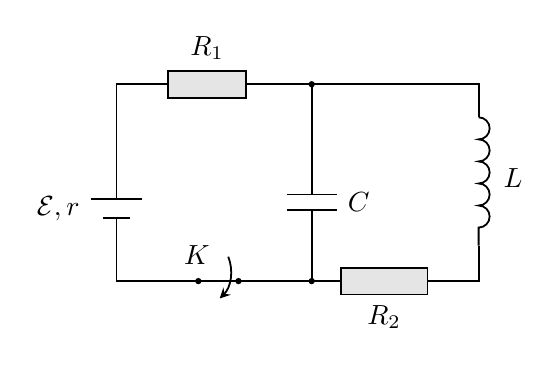
\begin{tikzpicture}[>=stealth,line width=.65pt]\draw (0,1.04)--(0,2.5)--(.65,2.5) (1.65,2.5)--(4.6,2.5)--(4.6,2.08) (4.6,.45)--(4.6,0)--(3.95,0) (2.85,0)--(1.55,0) (1.04,0)--(0,0)--(0,.8);\draw (2.48,2.5)--(2.48,1.1) (2.48,.9)--(2.48,0);\draw (-.32,1.04)--(.32,1.04) (-.17,.8)--(.17,.8) (2.16,1.1)--(2.8,1.1) (2.16,.9)--(2.8,.9);\draw[fill=gray!20](.65,2.33)rectangle(1.65,2.67) (2.85,-.17)rectangle(3.95,.17);\draw (4.6,2.08) arc(90:-90:.14) arc(90:-90:.14) arc(90:-90:.14) arc(90:-90:.14) arc(90:-90:.14) --(4.6,.45);\draw (1.04,0)--(1.55,0);\draw[->] (1.42,.31)arc(22:-45:.49);\foreach \p in {(1.04,0),(1.55,0),(2.48,0),(2.48,2.5)}{\fill \p circle(.04);}\node[left]at(-.34,.92){$\mathcal E,r$};\node[above]at(1.15,2.68){$R_1$};\node[below]at(3.4,-.18){$R_2$};\node[right]at(2.81,1){$C$};\node[right]at(4.79,1.31){$L$};\node[above]at(1.02,.08){$K$};\end{tikzpicture}\end{center}

Электрическая цепь состоит из источника питания с ЭДС $\mathcal{E} = 10\,\text{В}$ и внутренним сопротивлением $r = 1\,\text{Ом},$ двух резисторов с сопротивлениями $R_1 = 5\,\text{Ом}$ и $R_2 = 4\,\text{Ом},$ конденсатора электроёмкостью $C = 80\,\text{мкФ},$ катушки с индуктивностью $L = 200\,\text{мкГн}$ и замкнутого ключа К. Схема этой цепи показана на рисунке. Пренебрегая сопротивлением катушки, определите, какое количество теплоты Q выделится в резисторe $R_2$ в течение длительного времени после размыкания ключа К?
}{
\smallskip\noindent\textbf{Решение}\par
$1$.  До размыкания ключа через катушку течёт постоянный ток, сила которого, по закону Ома для замкнутой цепи, равна 

\[I = \frac{\mathcal{E}}{r + R_1 + R_2} .\]
 При этом напряжение на конденсаторе постоянно и равно падению напряжения на резисторе $R_2,$ поскольку конденсатор и ветвь цепи, содержащая последовательно соединённые резистор $R_2$ и идеальную катушку, соединены параллельно. Поэтому напряжение на конденсаторе равно $U_C = IR_2.$
$2$.  В замкнутом участке цепи, содержащем конденсатор, катушку и резистор $R_2,$ после размыкания ключа возникнут затухающие электромагнитные колебания. Спустя достаточно большое время они прекратятся. В процессе этих колебаний в резисторе $R_2,$ в соответствии с законом Джоуля-Ленца, будет выделяться количество теплоты.
$3$.  Из закона сохранения энергии, примененного для электрической цепи, следует, что к моменту полного затухания указанных колебаний выделившееся в резисторе $R_2$ количество теплоты Q будет равно сумме энергии, запасенной на момент размыкания ключа К в конденсаторе  $W_C= \frac{CU ^2 _C}{2} ,$ и энергии, запасённой в катушке  $W_L= \frac{LI ^2}{2} .$
$4$.  Подставляя в записанные формулы выражения для $U_{C}$ и I, с учётом численных значений физических величин, получим:

$Q=W_C + W_L= \frac{CU ^2 _C}{2} + \frac{LI ^2}{2} = \frac{CR ^2 _2 I ^2}{2} + \frac{LI ^2}{2} = \frac{I ^2 ( CR ^2 _2 + L )}{2} =$

$= \frac{\mathcal{E} ^2 ( CR ^2 _2 + L )}{2 ( r + R_1 + R_2 ) ^2} = \frac{10 ^2 \cdot ( 80 \cdot 10 ^{ - 6 } \cdot 4 ^2 + 200 \cdot 10 ^{ - 6 } )}{2 \cdot ( 1 + 5 + 4 ) ^2} =0{,}74\,\text{мДж}.$

Ответ: $Q= \frac{\mathcal{E} ^2 ( CR ^2 _2 + L )}{2 ( r + R_1 + R_2 ) ^2} =0{,}74\,\text{мДж}.$
}

\end{document}
